\documentclass{article}
\usepackage{graphicx}
\usepackage{amsmath,amssymb,amsfonts,amsthm,mathtools} % Mathematik
\usepackage{subfigure} 
\usepackage{color}

\title{Sheet 2 - Answers}
\author{Timm \& Boris}

\begin{document}
\maketitle

\section*{Task: 1}

\begin{figure}[htbp]
  \centering
    \includegraphics[width=0.50\textwidth]{../Task01/sh2_task1_mean_estimates_plot.eps}
			\caption{Plot of call option pricing mean estimates against different values of $\sigma$.}
\end{figure}

\section*{Task: 2}
Seems like the variance increases with $\delta t$ and the mean has a slow increasing rate.

\begin{figure}[htbp]
  \centering
     \includegraphics[width=0.40\textwidth]{../Task02/sh2_task2_variance_estimates_plot.eps}
   \caption{Plot of call option pricing mean and variance estimates against different values of $\Delta t$.}
\end{figure}

\section*{Task: 3}

\noindent We have:
\begin{align*}
 \mathbb{E}[V_{\text{call}}(S_T,0)] =& \frac{1}{\sqrt{2 \pi}} \int_{\chi}^\infty f_{\text{call}}(s)e^{-\frac{s^2}{2}}ds\\
  =&\frac{1}{\sqrt{2 \pi}} \int_{\chi}^\infty \left( S(0)e^{(\mu-\frac{1}{2}\sigma^2)\cdot T+\sigma\sqrt{T}s}-K\right)e^{-\frac{s^2}{2}}ds
\end{align*}
With:
\begin{align*}
 \chi = \frac{1}{\sigma \sqrt{T}}\left(\log\left(\frac{K}{S_0}\right)-\left(\mu-\frac{\sigma^2}{2}\right)T\right)
\end{align*}
It follows:
\begin{align*}
 \mathbb{E}[V_{\text{call}}(S_T,0)] = & \frac{1}{\sqrt{2 \pi}} \int_{\infty}^{-\chi} S(0)e^((\mu-\frac{1}{2}\sigma^2)\cdot T-\sigma\sqrt{T}s)e^{-\frac{s^2}{2}}ds\\
                                      & - \frac{K}{\sqrt{2 \pi}} \int_{\infty}^{-\chi} e^{-\frac{s^2}{2}}ds\\
                                    = & S(0) e^{(\mu-\frac{1}{2}\sigma^2)\cdot T}\frac{1}{\sqrt{2 \pi}} \int_{\infty}^{-\chi} e^{-\frac{s^2}{2}-\sigma\sqrt{T}s}ds - K \Phi(-\chi)\\
                                    = & S(0) e^{\mu T}\textcolor{red}{e^{-\frac{1}{2}\sigma^2 T}}\frac{1}{\sqrt{2 \pi}} \int_{\infty}^{-\chi} e^{-\frac{1}{2}(s+\sigma\sqrt{T})^2\textcolor{red}{+\frac{1}{2}\sigma^2 T}}ds - K \Phi(-\chi)\\
                                    = & S(0) e^{\mu T} \Phi(\sigma \sqrt{T} - \chi) - K \Phi(-\chi)
\end{align*}
{\flushright{$\qed$}}

\section*{Task: 4}  %///////////////////////////////////
\begin{figure}[htbp]
  \centering
     \includegraphics[width=0.50\textwidth]{../Task04/sh2_task4_plot.eps}
   \caption{Plot of call option pricing mean and variance estimates against different values of $\Delta t$.}
\end{figure}

\section*{Task: 5}

\noindent To proof:
\begin{align*}
 \frac{1}{\sqrt{2 \pi}} \int_{-\infty}^\infty f(s)e^{-\frac{s^2}{2}}ds =& \int_{0}^1 f(\Phi^{-1}(t))dt
\end{align*}
Proof:
\begin{align*}
 \frac{1}{\sqrt{2 \pi}} \int_{-\infty}^\infty f(s)e^{-\frac{s^2}{2}}ds =& \lim_{a\rightarrow \infty}\int_{-a}^a f(s) \phi '(s)ds\\
  =& \lim_{a\rightarrow \infty}\int_{\Phi(-a)}^{\Phi(a)} f(\Phi^{-1}(t)) dt\\
  =& \int_{0}^{1} f(\Phi^{-1}(t)) dt
\end{align*}
With substitution $s\rightarrow \Phi^{-1}(t)$.
{\flushright{$\qed$}}

\section*{Task: 6}

The nodes in level $l$ are $\frac{i}{2^l}$ for $i=1,...,2^l-1$.
In level $l + 1$ they are $\frac{i}{2^{l+1}}$ for $i=1,...,2^{l+1}-1$.\\
Thus the level $l$ nodes are the even nodes in level $l+1$.

\section*{Task: 7}

\noindent Gauss Legendre quadrature is a quadrature rule where the evaluation points are the roots of the
$n$-th Legendre polynomial and the weights are the integrals of the corresponding Lagrange polynomials of degree $n$ over the integration domain.\\

\noindent Legendre polynomial:
\begin{align*}
 P_n(x)&=\frac{1}{2^n}\sum_{k=0}^n {n \choose k}^2 (x-1)^{n-k}(x+1)^k \\
 &= \sum_{k=0}^n {n \choose k}{-n-1 \choose k}\left(\frac{1-x}{2}\right)^k
\end{align*}

\noindent Lagrange polynomials:
\begin{align*}
 L_{i,n}(x)=\prod_{j=0 \atop j\neq i}^n \frac{x-x_j}{x_i-x_j}
\end{align*}
(Where $x_i$ are the evaluation points.)

\subsection*{Level behavior}
We concluded that the behavior of the nodes does not change likewise as in the other integrating methods. We see in the graphic below that the roots of the polynomials do not cross.
\begin{figure}[htbp]
  \centering
     \includegraphics[width=1.00\textwidth]{../Task07/LevelBehavior.eps}
   \caption{LevelBehavior}
\end{figure}

\section*{Task: 8}

Analogous to the trapezoidal rule the even nodes of level $l+1$ are the nodes of level $l$.

\section*{Task: 9}

\begin{figure}[htbp]
  \centering
     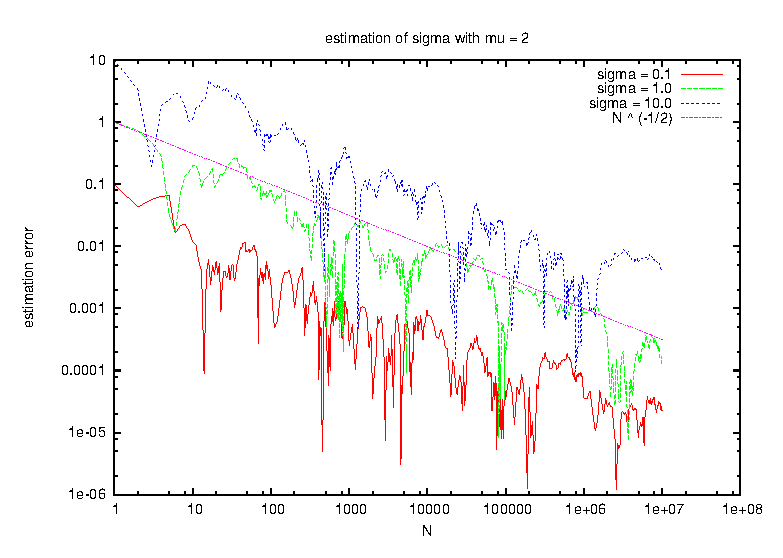
\includegraphics[width=0.50\textwidth]{../Task09/task9_convergence_plot.eps}
   \caption{Plot of numerical integration errors (relative) for function $1+\exp\left(\frac{1}{2}x\right)$.}
\end{figure}

\section*{Task: 10}

\begin{figure}[htbp]
  \centering
     \includegraphics[width=0.50\textwidth]{../Task10/task10_convergence_plot.eps}
   \caption{Plot of numerical integration errors (relative) for the expectation of the call option.}
\end{figure}

\end{document}